\section{Appendix: Directional Supporting Evidence}

\textit{The following figures provide supporting diagnostic evidence for the strategic audit, preserving the complete research coverage of the 01--04 exploratory directions without diluting the core forensic narrative.}

\subsection{A. Product \& Market Dominance (Direction 01)}
\begin{figure}[!htbp]
\centering

\includegraphics[width=0.85\textwidth]{figures/margin_by_size.png}
\caption{\textbf{Sizing margin pockets:} The L/XL size bands hold the highest absolute unit profitability in the streetwear assortment, indicating that the business should over-index supply chain planning toward larger sizes.}
\label{fig:appendix_margin_size}
\end{figure}

\begin{figure}[!htbp]
\centering
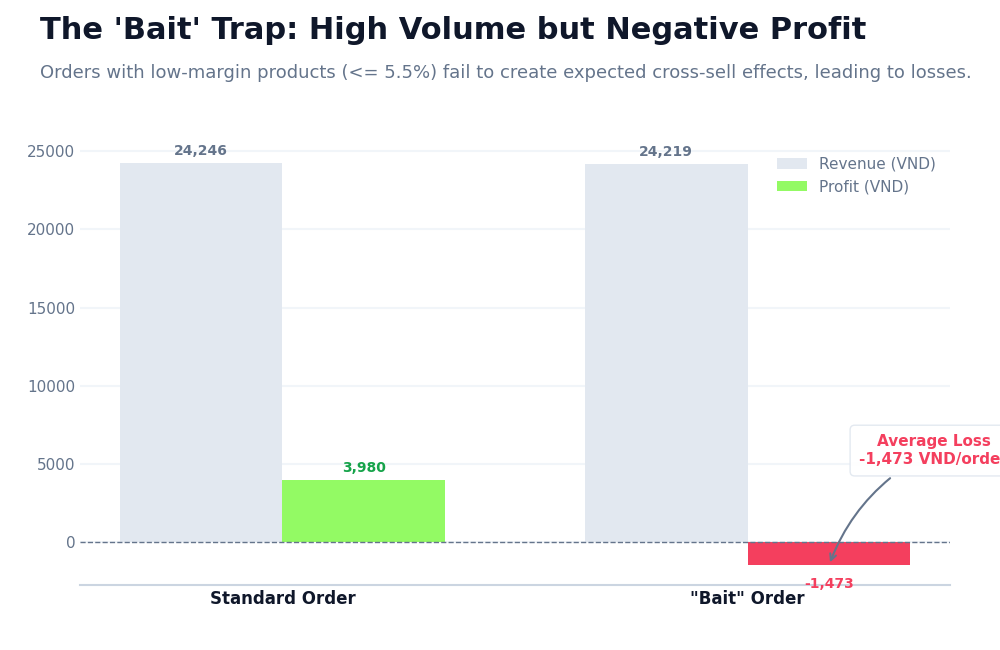
\includegraphics[width=0.85\textwidth]{figures/1_loss_leader_trap.png}
\caption{\textbf{Loss Leader Trap:} Low-margin SKUs generate revenue but destroy basket profit, proving that traffic products need bundling or margin-floor guardrails.}
\label{fig:loss_leader_trap}
\end{figure}

\begin{figure}[!htbp]
\centering

\includegraphics[width=0.85\textwidth]{figures/3_product_lifecycle.png}
\caption{\textbf{R\&D Evolution:} Newest product iterations (suffix > 70) generate 64\% more average revenue per SKU than original classic models, proving that active product innovation outpaces passive restocking.}
\label{fig:appendix_rd}
\end{figure}

\FloatBarrier

\subsection{B. Customer Lifecycle \& Acquisition (Direction 02)}
\begin{figure}[!htbp]
\centering
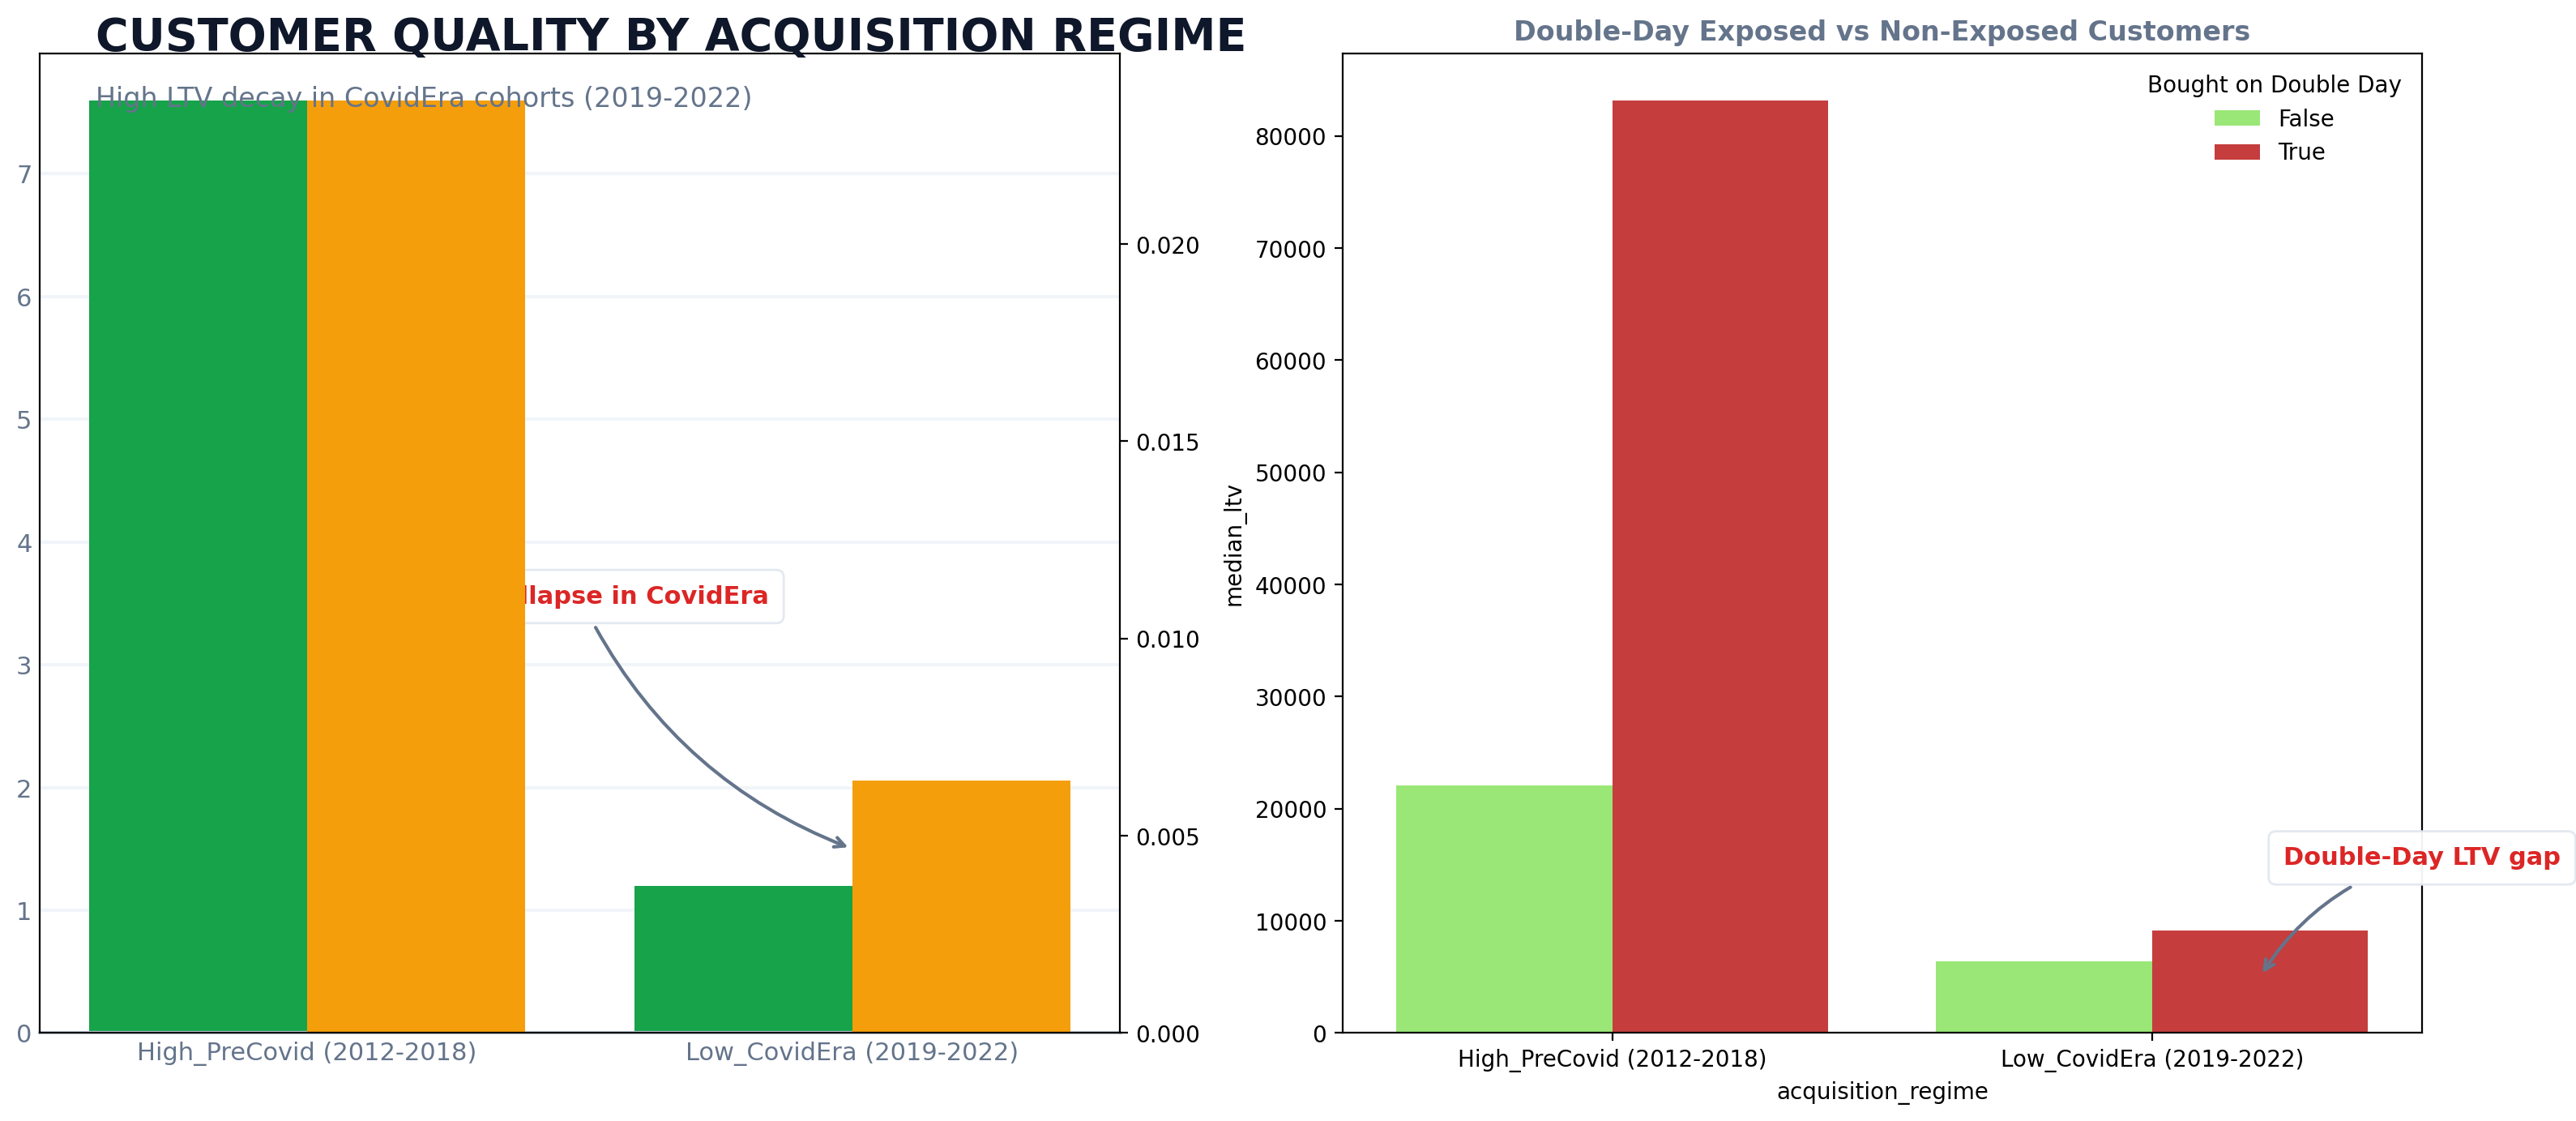
\includegraphics[width=0.85\textwidth]{figures/regime_double_day_ltv.png}
\caption{\textbf{Customer Quality Shift:} Post-2018 cohorts (the Double Day discount regime) show structurally weaker repeat value and lower baseline loyalty than the original community-driven cohorts.}
\label{fig:appendix_customer_quality}
\end{figure}

\begin{figure}[!htbp]
\centering

\includegraphics[width=0.85\textwidth]{figures/acquisition_efficiency.png}
\caption{\textbf{Acquisition Efficiency:} Channel performance diverges materially, so CAC targets should be calibrated by channel quality rather than blended across all new customers.}
\label{fig:appendix_acquisition_efficiency}
\end{figure}

\begin{figure}[!htbp]
\centering

\includegraphics[width=0.85\textwidth]{figures/order_frequency_dist.png}
\caption{\textbf{Single-Order Problem:} The order-frequency distribution confirms that the loyalty collapse is not abstract — it is visible as a large single-purchase customer base.}
\label{fig:appendix_order_freq}
\end{figure}

\FloatBarrier

\subsection{C. Operational Friction \& Leakage (Direction 03)}
\begin{figure}[!htbp]
\centering

\includegraphics[width=0.85\textwidth]{figures/4_tet_effect.png}
\caption{\textbf{Seasonal Operations:} The Tet demand curve proves the necessity of a T-30 supply staging strategy before the holiday logistics network freezes.}
\label{fig:appendix_tet}
\end{figure}

\begin{figure}[!htbp]
\centering

\includegraphics[width=0.85\textwidth]{figures/returns_bar.png}
\caption{\textbf{Return Drivers:} "Wrong size" overwhelmingly dominates return reasons across all categories. Fixing sizing accuracy is the fastest controllable path to operational margin recovery.}
\label{fig:appendix_returns}
\end{figure}

\begin{figure}[!htbp]
\centering

\includegraphics[width=0.85\textwidth]{figures/return_friction_matrix.png}
\caption{\textbf{Return Friction Matrix:} Return causes differ by category, so sizing, quality-control, and customer-education fixes should be category-specific rather than universal.}
\label{fig:appendix_return_matrix}
\end{figure}

\begin{figure}[!htbp]
\centering

\includegraphics[width=0.85\textwidth]{figures/inventory_risk_analysis.png}
\caption{\textbf{Inventory Risk:} High-demand SKUs still face stockout or replenishment mismatch, turning seasonal peaks into missed-revenue events.}
\label{fig:appendix_inventory_risk}
\end{figure}

\FloatBarrier

\subsection{D. Financial \& Payment Dynamics (Direction 04)}
\begin{figure}[!htbp]
\centering

\includegraphics[width=0.85\textwidth]{figures/5_campaign_roi.png}
\caption{\textbf{Campaign ROI:} Spring Sale creates profitable lift, while Year-End Sale destroys both revenue and margin, proving that campaign mechanics matter more than discount volume.}
\label{fig:appendix_campaign}
\end{figure}

\begin{figure}[!htbp]
\centering

\includegraphics[width=0.85\textwidth]{figures/promo_urgency_stackability.png}
\caption{\textbf{Promo Urgency \& Stackability:} Final-window urgency can lift conversion, but stackable discounts risk margin dilution beyond the safe threshold.}
\label{fig:appendix_stackability}
\end{figure}

\begin{figure}[!htbp]
\centering

\includegraphics[width=0.85\textwidth]{figures/revenue_margin_trend.png}
\caption{\textbf{Margin Compression:} While top-line revenue has grown consistently, gross margin percentage has compressed, demonstrating that the current acquisition engine relies on unsustainable promotional pricing.}
\label{fig:appendix_revenue_margin}
\end{figure}

\FloatBarrier
